\section{Présentation de la situation initiale}
\subsection{État de l'art}
\subsubsection{Architecture backend}
Parmi les solutions informatiques que CLARISYS INFORMATIQUE édite, nous nous intéressons, 
dans ce rapport, au progiciel MCA « Manager Connexion Automate ».

MCA est un middleware\footnote[2]{En architecture informatique, un middleware ou intergiciel est 
un logiciel tiers qui crée un réseau d'échange d'informations entre différentes applications informatiques.}
expert, conçu en application web, accessible via un navigateur web. 
Il assure le pilotage et le traitement de l'activité analytique d'un laboratoire, y compris 
celle de bactériologie. Il se charge également d’établir les différents types de connexions 
entre les différents analyseurs et de traiter les envois de demandes d’analyse vers ces derniers 
et le retour de résultats.

MCA est développé en utilisant le Framework Django\footnote[3]{Django est un cadre de 
développement web open source en Python. Il a pour but de rendre le développement web 2.0 simple et rapide.}
pour sa partie « Backend\footnote[4]{En informatique, un back-end est un terme désignant un étage de sortie 
d'un logiciel devant produire un résultat. On l'oppose au front-end qui lui, est la partie visible.} » ; 
En effet, il s’agit d’un Framework robuste, qui, s’il est correctement exploité, 
permet de produire un projet solide en très peu de temps. Malgré le fait qu’il ait 
vu le jour en 2003, Django figure aujourd’hui largement parmi les plus utilisés. 
Régulièrement mis à jour, c’est un outil qui, pour le moment, rivalise aisément avec 
la plupart des autres outils existants.
\begin{figure}[hp]
    \centering
    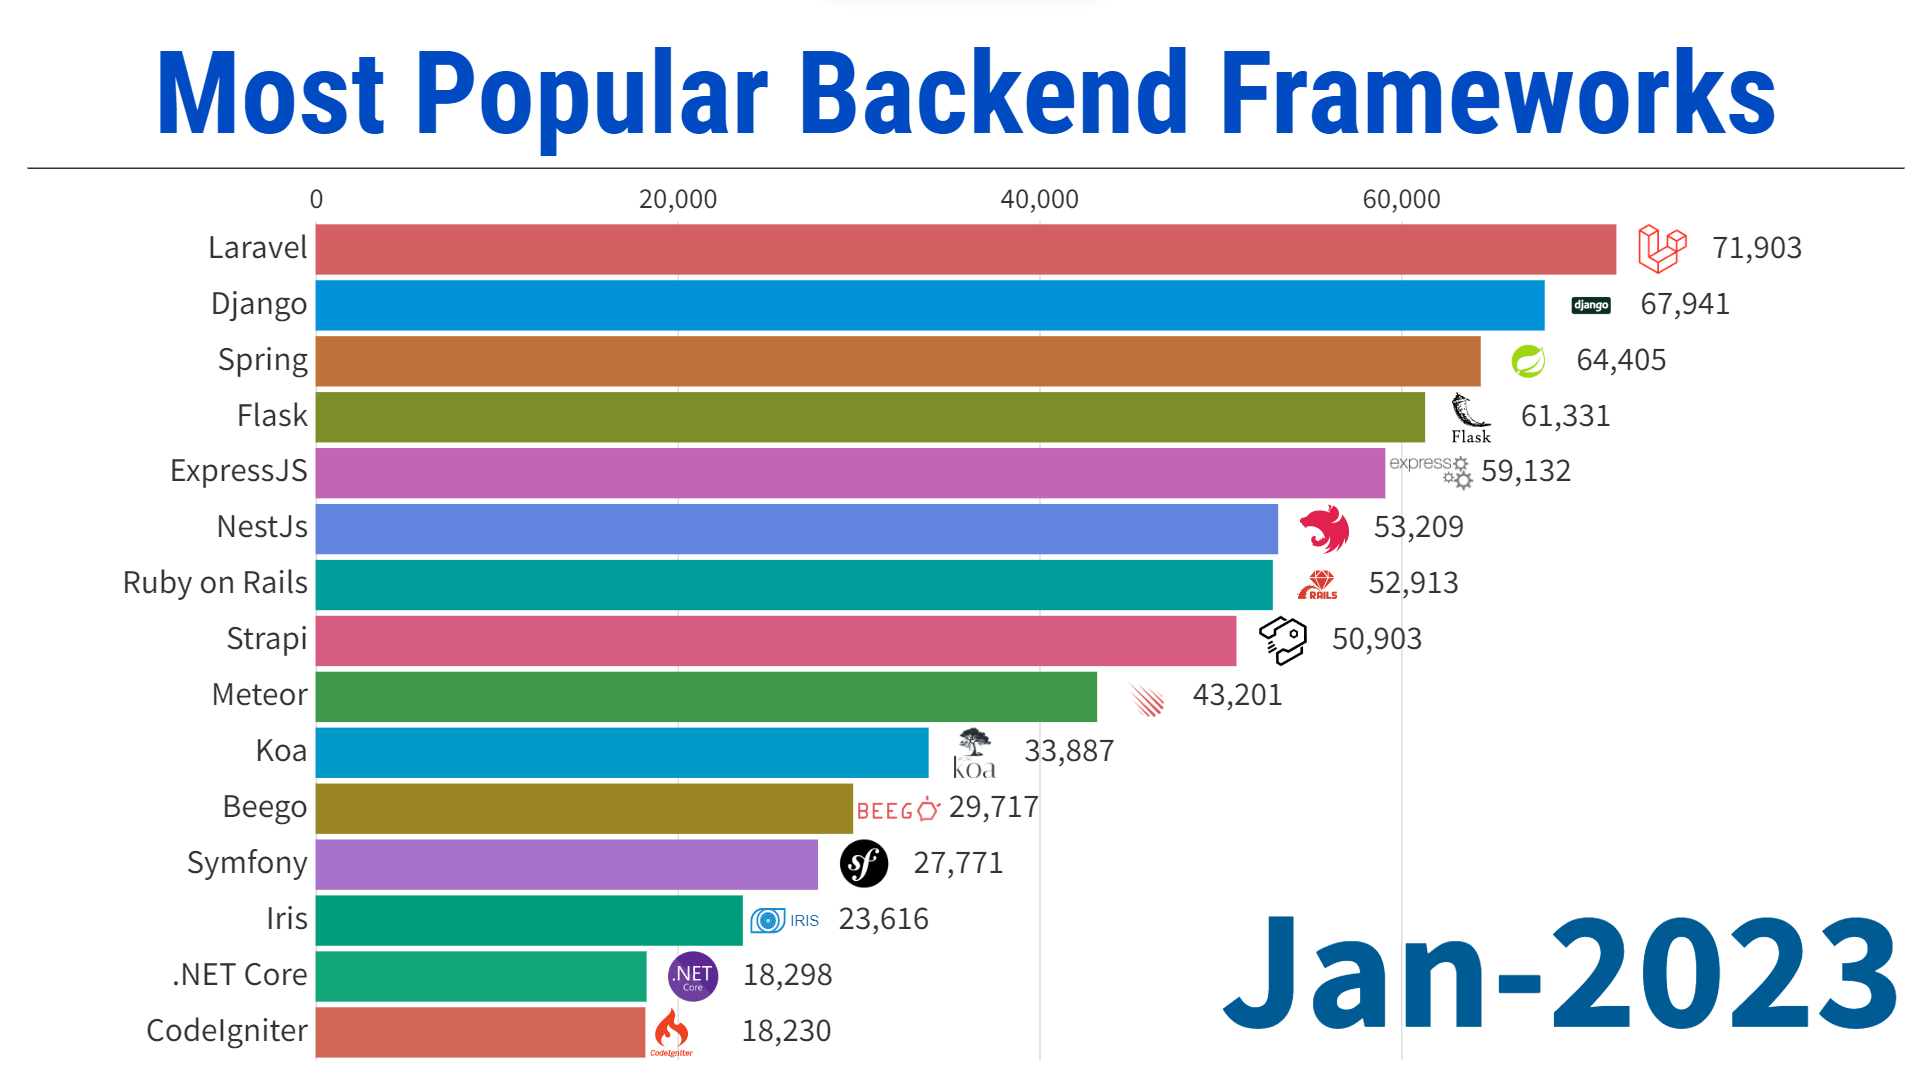
\includegraphics[width=400pt,height=200pt]{images/frameworks_2023.png}
    \caption{Frameworks back end les plus populaires en Janvier 2023}
\end{figure}
\pagebreak

Django possède de nombreux avantages. Il est facile à prendre en main, ce qui représente un avantage 
pour de nombreux développeurs. Riche en fonctionnalités, Django peut donc s’adapter à n’importe 
quel type de projet web. 
Autre élément crucial pour CLARISYS INFORMATIQUE, il s’agit d’un outil sécurisé, qui aide ses 
utilisateurs à éviter de nombreux problèmes de sécurité comme l’injection SQL\footnote[5]{La faille SQLi, 
abréviation de SQL Injection, soit injection SQL en français, est un groupe de méthodes d'exploitation
 de faille de sécurité d'une application interagissant avec une base de données.}. Django repose sur 
l’architecture MVT (Model, View, Template), elle-même inspirée du modèle MVC (Model, View, Controler) 
plus largement connu et utilisé par la plupart des autres frameworks web.
\begin{figure}[hp]
    \centering
    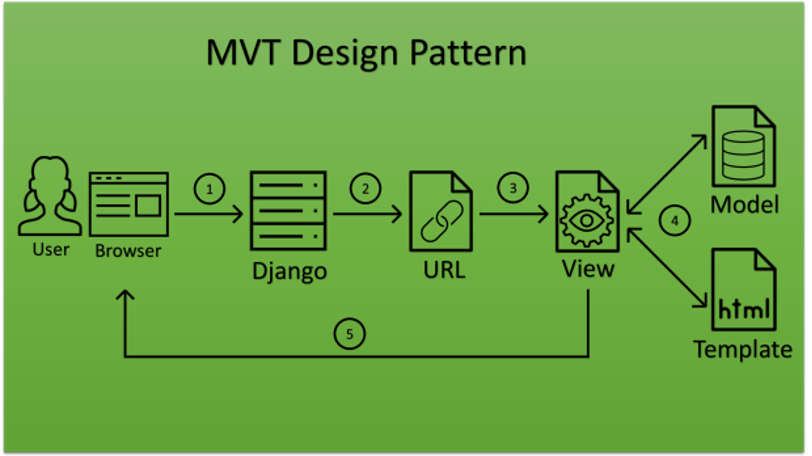
\includegraphics[width=400pt,height=200pt]{images/django_pattern.png}
    \caption{Schéma de l'architecture MVT de Django}
\end{figure}

L’architecture MVT de Django est composée de trois couches :\\
o	Le Modèle : Le Modèle définit la structure des données et les représente sous forme d’objets ou 
classes d’objets. C’est la couche qui interagit avec la base de données via un ORM\footnote[6]{ORM signifie 
Object-Relational Mapping. Un ORM est un ensemble de classes permettant de manipuler les tables d'une 
base de données relationnelle comme s'il s'agissait d'objets.}.\\
o	La Vue : La Vue contrôle ce que l’utilisateur peut consulter. Elle récupère les requêtes web et 
renvoie la réponse correspondant à chaque requête.\\
o	Le Template : Le Template définit l’interface graphique que consulte l’utilisateur.
Il permet de contrôler l’interaction avec l’utilisateur et gère la façon dont la réponse à une 
requête est retournée à celui-ci.\\
\pagebreak

\subsubsection{Architecture REST}
Dans l’architecture Backend de MCA, nous pouvons constater qu’au-delà de l’architecture classique de Django, 
il existe de nombreux modules applicatifs de MCA qui sont fournis aussi en « REST API\footnote[7]{L'API REST 
(Representational State Transfer - Application Program Interface) est un style architectural qui permet 
aux développeurs de créer des services web. REST utilise des méthodes HTTP pour récupérer et publier des 
données entre un appareil client et un serveur.}». 
En effet, il s’agit de la librairie Django REST Framework écrite en Python. 
DRF se base sur le Framework Django pour concevoir des APIs REST. L’avantage principal de l’architecture 
REST de Django REST Framework comparé à Django MVT, est que l’architecture REST permet de séparer la partie 
Backend (la partie concernant le serveur, les données, l’authentification…) de la partie Frontend\footnote[8]{Le développement frontend correspond aux productions HTML, CSS et JavaScript 
d’une page internet ou d’une application qu’un utilisateur peut voir et avec lesquelles il peut interagir 
directement.} (la partie visible de l’application).
REST étant une approche distribuée, les applications client et serveur doivent être complètement découplées 
(indépendantes) les unes des autres, quel que soit l'endroit d'où proviennent les demandes afin de minimiser 
les interactions.

La seule information que l'application client doit connaître est l'identifiant de ressource uniforme (URI) 
de la ressource demandée. Elle ne peut interagir avec l'application serveur d'aucune autre manière.

Toute demande effectuée par un consommateur sera, soit acceptée, soit rejetée par le serveur. De même, 
une application serveur doit permettre aux applications clientes d'accéder aux données demandées via 
HTTP sans aucune modification.

\begin{figure}[hp]
    \centering
    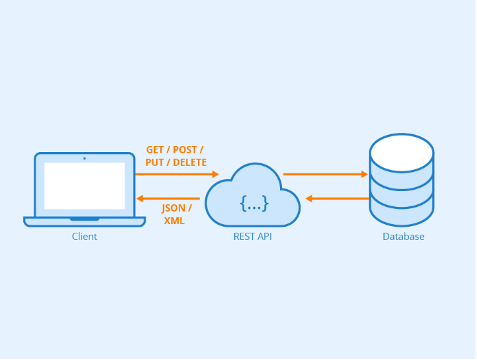
\includegraphics{images/arch_rest.png}
    \caption{Schéma de l'architecture REST API}
\end{figure}

Ce découplage de deux parties de l’architecture d’une application web permet d’intégrer plusieurs clients 
qui peuvent consommer le REST API.
Le rôle premier d’une API REST est de servir d’intermédiaire entre le client et le serveur. C’est-à-dire 
que c’est elle qui réceptionne les requêtes émises par le client, les transmet à l’entité demandée au serveur, 
prend les réponses données par ce dernier puis les retransmet au client.
En effet, en faisant appel à une URI, nous pouvons récupérer une quantité importante de données. Cela offre 
de grands avantages pour les deux parties : les clients peuvent augmenter la performance de leurs applications
 et de leurs sites. Quant aux serveurs, ils gagnent en performance car ils ne sont plus amenés à charger 
 l’interface graphique de l’application web. En revanche, le serveur s’occupe de transmettre les données 
 demandées en format JSON\footnote[9]{JavaScript Object Notation est un format de données textuelles dérivé de
la notation des objets du langage JavaScript. Il permet de représenter de l’information structurée.} ou 
XML\footnote[10]{XML (eXtensible Markup Language) est en quelque sorte un langage HTML amélioré permettant 
de définir de nouvelles balises. Il s'agit effectivement d'un langage permettant de mettre en forme des
documents grâce à des balises.}  par la requête de client et ce dernier s’occupe de l’affichage graphique.
Il faut également savoir qu’une seule API REST peut facilement alimenter plusieurs applications. Ce qui veut 
dire que le temps et la ressource utilisés sont fortement réduits.
\begin{figure}[hp]
    \centering
    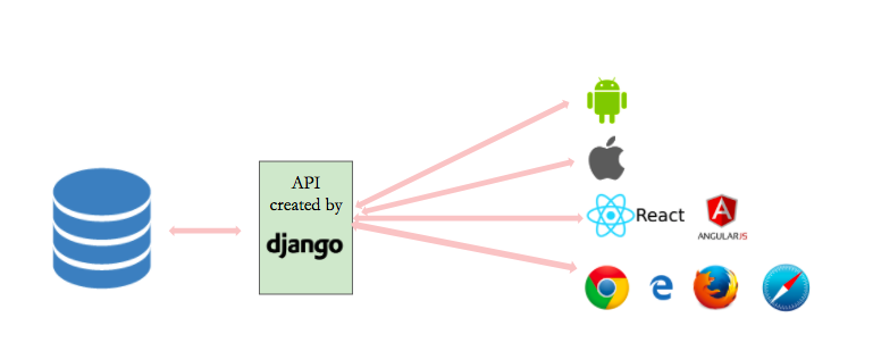
\includegraphics{images/rest_api_pres.png}
    \caption{Description d'un REST API}
\end{figure}

De plus, c’est une manière idéale de sécuriser les applications pour les deux parties concernées car 
les interactions directes pouvant entrainer de fausses manipulations sont évitées au maximum.
\pagebreak
\subsubsection{Le modèle de maturité de Richardson}
Développé par Leonard Richardson, ce modèle permet de découper les contraintes de REST en trois étapes 
principales afin de mettre en application la théorie de REST en tant que service web.
\begin{figure}[hp]
    \centering
    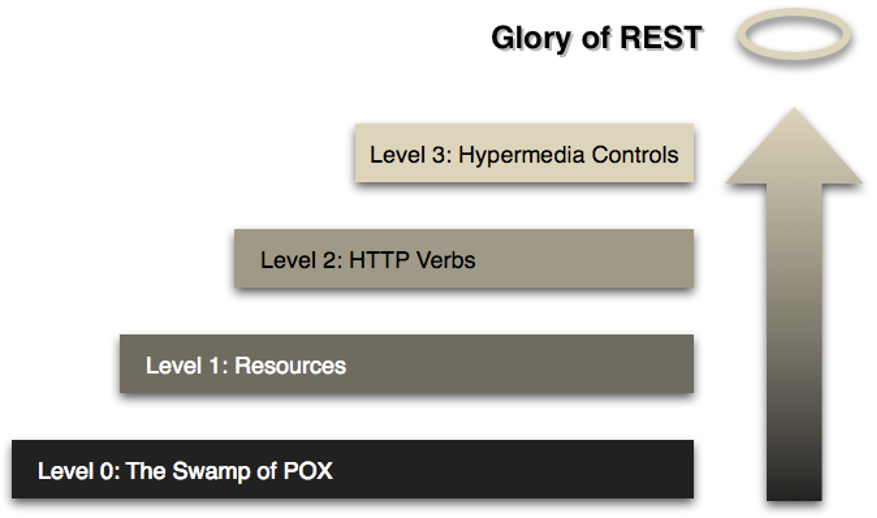
\includegraphics{images/richardson.png}
    \caption{Le modèle de maturité de Richardson}
\end{figure}

Dans son article intitulé « REST APIs must be hypertext-driven » \cite{rest_hyper}, 
Roy T. Fielding\footnote[11]{Roy Thomas Fielding : (né en 1965) est un informaticien américain, 
l'un des principaux auteurs de la spécification HTTP et à l'origine du style architectural 
Representational State Transfer (REST). Il fait autorité en matière d' architecture de réseau 
informatique et a cofondé le projet Apache HTTP Server .} a décrit les points fondamentaux 
d’un REST API après avoir 
indiqué que les principes de REST ne sont pas toujours respectés. 
Nous pouvons trouver parmi ces points la notion de « Hypermedia-drive API’s » 
ou plus précisément HATEOAS (Hypermedia as the Engine of Application State).
Pour bien utiliser l’HATEOAS, il est important de comprendre deux principes essentiels :\\
-	les URLs Immutables, ou les liens qui retournent toujours les mêmes ressources\\
-	la navigation API, ou la modélisation en arbre avec des transitions.\\
-	Les  states  sont les pages web et les transitions sont les liens hypertextes.\\ 

L’idée derrière le HATEOAS est donc très simple. Pour chaque réponse du serveur nous incluons des 
liens vers les prochaines requêtes pour explorer les autres ressources.
\pagebreak

Prenons l’exemple d’une réponse JSON d’un serveur suite à une requête de récupération des utilisateurs (Réponse classique non-HATEOAS).
\begin{figure}[hp]
    \centering
    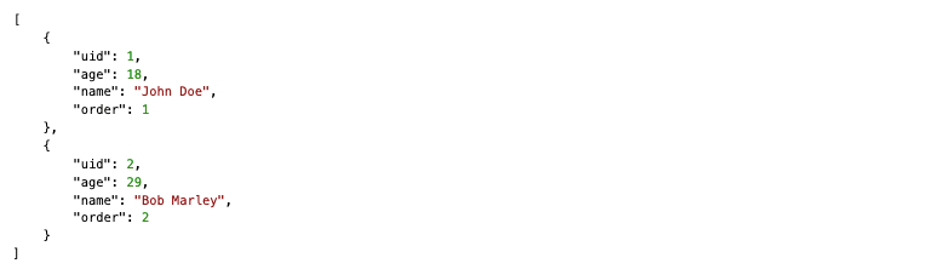
\includegraphics{images/nohtaos.png}
\end{figure}

Et si un client qui consomme cet API veut en savoir plus sur les utilisateurs ? 
Doit-il préparer à l’avance ses URLs qui mènent vers les ressources de détails de chaque utilisateur ? 
Et si l’API évolue au cours du temps et les URLs changent ? Que faire ?

La solution serait donc que l’API fournisse au client des liens dans la réponse, 
semblables à des hyperlinks dans un site web. Le premier avantage est que le client sera 
complètement dissocié de l’API de service et qu’il n’a pas à hard-coder les URLs pour interagir avec 
l’API et l’application state.
\begin{figure}[hp]
    \centering
    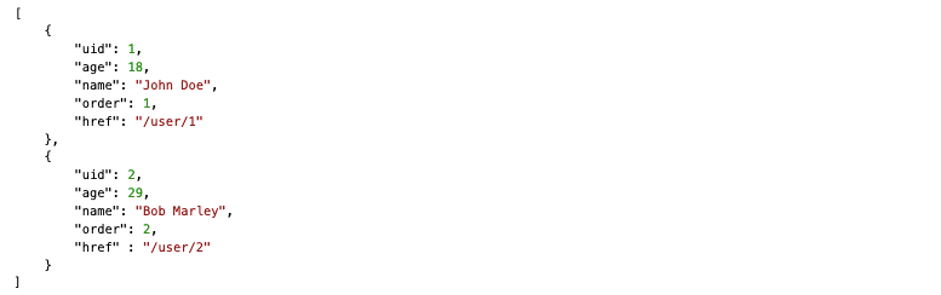
\includegraphics{images/htaos.png}
\end{figure}

C’est exactement la même réponse qu’avant, mais avec un champ href en plus, contenant un lien direct vers 
les ressources détails d’un utilisateur. 

Donc, avec cette idée, le client n’a pas à se rappeler des valeurs des urls, notamment quand 
l’API utilise les URLs immutables qui changent à chaque révision. La solution est donc d’ajouter 
des informations supplémentaires dans notre réponse JSON via l’attribut href qui a comme tâche de
 nommer les URLs.

Ainsi, notre réponse embarque toutes les URLs permettant d’explorer l’API pour un utilisateur 
et l’attribut href permet de donner un sens aux URLs et facilite la gestion côté client.
\pagebreak

Les avantages des HATEOAS sont nombreux : 

o	Réduction des erreurs de codage - Côté client : En raison de l'accent mis sur l'utilisation des URI 
(identificateurs de ressources uniques), environ 90\% des bogues peuvent être éliminés grâce à HATEOAS. 
En général, les erreurs sont commises en omettant des segments de chemin d'accès ou en les plaçant dans 
le mauvais ordre. Parfois, même les codeurs oublient de coder les URL. Ces erreurs humaines courantes peuvent
 être minimisées en utilisant une approche HATEOAS\\

o	Mise à niveau détaillée de l'application sans rupture du client : les clients d'une API REST sont 
généralement programmés avec certaines hypothèses concernant le fonctionnement du système et ses limites. 
Les API peuvent évoluer assez rapidement si le développeur documente correctement une restriction à laquelle 
il faut prêter attention et cibler spécifiquement certains aspects du système. Cela s'accompagne d'une 
logique solide côté serveur pour l'ajout de choses à un stade ultérieur. Un bon développeur peut également 
s'assurer que tout cela ne perturbe pas les comportements précédemment codés. Grâce à cette approche, les 
API peuvent évoluer assez rapidement\\

Cela permet également de s'assurer que tous les clients restent en état de marche. 
Elle permet également de réduire la charge de travail du développeur, en évitant de 
multiples versions d'une API sur le serveur. C'est sans doute l'un des principaux avantages 
de la mise en œuvre d'API conforme à HATEOAS.
\pagebreak

\subsubsection{Docker}
Au-delà du Framework Django, qui donne un cadre pour le développement, MCA utilise d’autres technologies, 
notamment la plateforme de conteneurs Docker qui a récemment été mise en place afin de simplifier son 
installation.

Docker est une technologie qui permet de distribuer et de déployer des application en les plaçant dans 
des conteneurs qui se comportent comme des machines virtuelles. 

A la différence de ces dernières, les conteneurs docker s'exécutent nativement sur les systèmes et sont 
donc très efficaces en ressources utilisées. Ils sont auto-suffisants, ce qui signifie qu'ils contiennent
 tout ce dont l'application a besoin pour fonctionner, sans faire d'hypothèse sur la configuration de la
  machine qui les héberge.

Docker permet donc de rassembler dans un conteneur l'ensemble des fichiers et services dont l’application a
 besoin pour fonctionner.
 \begin{figure}[hp]
    \centering
    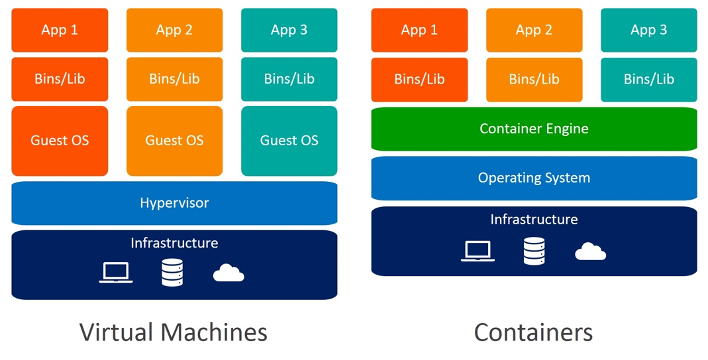
\includegraphics{images/docker.png}
    \caption{Schéma simplifié d’une application virtualisée VS application conteneurisée}
\end{figure}

Lancé en 2013, Docker permet de facilement créer des conteneurs et des applications basées sur les conteneurs. Même s’il existe d’autres solutions, Docker est largement plus utilisé, notamment car il est plus facile à utiliser et à déployer que ses concurrents. 

Ainsi, grâce à la conteneurisation, l’installation de MCA est devenue bien plus facile puisqu'il suffit d’effectuer quelques commandes pour pouvoir accéder à un environnement complet ainsi qu’une base de données et un logiciel fonctionnel. Cela permet également au développeur de créer, supprimer et recréer des conteneurs aisément.
\pagebreak

\subsubsection{Architecure Frontend}
Au cours de la vie de MCA, l’interface graphique a subi plusieurs 
refactorisations\footnote[12]{La refactorisation ou le  réusinage de code est l'opération consistant 
à retravailler le code source d'un programme informatique sans toutefois y ajouter des fonctionnalités 
ni en corriger les anomalies} concernant les 
technologies du Frontend. En effet, le développement Frontend a connu une forte hausse notamment 
ces dix dernières années.

 Ainsi, les technologies et les Frameworks aident les développeurs à accélérer le développement 
 et la mise en forme des interfaces des applications web grâce à des écosystèmes robustes.

Les premières versions de MCA n’utilisaient pas de Frameworks de Frontend et se contentaient de 
la traditionnelle association HTML, CSS, JavaScript. Depuis, en vue d’optimiser l’application ainsi que
 l’expérience utilisateur, l’équipe technique de Clarisys Informatique a étudié l’avantage d’inclure le 
 Frontend dans un Framework plus moderne et performant.

Les Frameworks de Frontend permettent aux développeurs de se concentrer uniquement 
sur la partie métier puisque toutes les couches techniques sont déjà intégrées dans le Framework.
 C’est un gain de temps pour le développement et donc aussi pour le projet.

L’architecture permet la séparation des couches techniques logiques afin de faciliter le développement 
en équipe, la maintenance et l’évolution. Par exemple, un développeur ne travaillera pas sur la même 
couche qu’un intégrateur. Cela permet de paralléliser les tâches et d’éviter les conflits dans la 
gestion des sources.

La maintenance et l’évolution du framework sont gérées par l’organisme fondateur. Ce n’est pas l’équipe 
de développement qui aura la charge de le maintenir. Tout ce temps économisé pourra être dépensé en 
recherche et développement et apporter de la valeur ajoutée au projet.

Le seul inconvénient réel qui pourrait freiner l’utilisation d’un Framework est le temps d’apprentissage. 
C’est le prix à payer car la prise en main peut parfois s’avérer fastidieuse. Mais une fois le Framework 
maîtrisé, elle ne peut qu’améliorer les développements.
\pagebreak

Les critères à prendre en compte dans le choix avant même de tester le framework (ces critères valent pour le choix de n’importe quelle technologie) :\\
•	La maturité du framework : il vaut mieux choisir des technologies qui sont là depuis 
longtemps et qui ont déjà fait leurs preuves plutôt qu’un  « petit nouveau » qui va peut-être devoir
 résoudre des défauts de jeunesse. Autre avantage : une technologie mature a eu le temps de rassembler
  une grande communauté d’utilisateurs/développeurs prête à venir en aide aux membres en difficultés 
  grâce aux forums de discussion, à la documentation, aux ressources\\
•	La rapidité de mise en œuvre, c’est-à-dire le temps nécessaire pour l’installation du 
framework et celui entre l’installation et le moment où le framework est opérationnel\\
•	La courbe d’apprentissage, qui est le temps nécessaire pour apprendre à maîtriser le framework\\
•	L’acceptation par le framework des conventions de programmation et des best practices\\
•	La capacité du framework à s’adapter à l’évolution des technologies : autrement dit, mature 
ne veut pas dire « fossilisé ».  Il faut que le framework évolue avec son temps\\
•	La capacité du framework à s’adapter à la charge, c’est-à-dire à l’augmentation du nombre 
d’utilisateurs\\
\begin{figure}[hp]
    \centering
    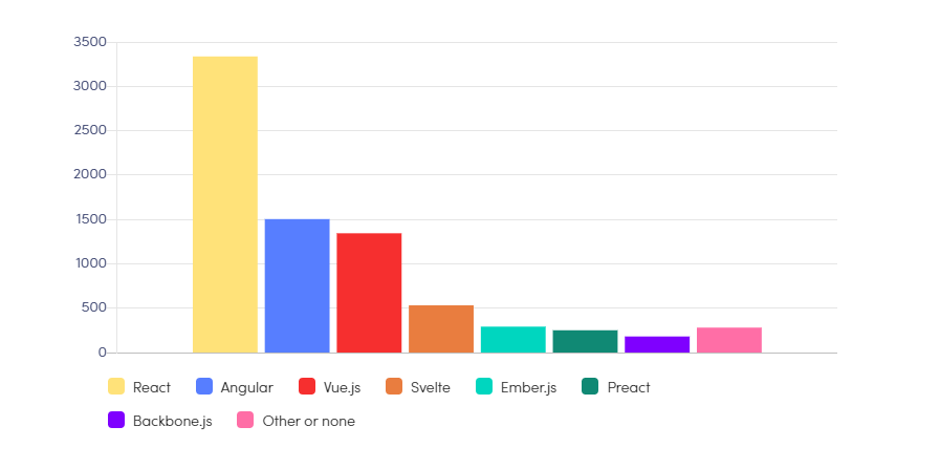
\includegraphics{images/frontend_frameworks.png}
    \caption{Frameworks Frontend les plus populaires en Janvier 2022}
\end{figure}
\pagebreak

\subsubsection{VueJS}
\begin{figure}[hp]
    \centering
    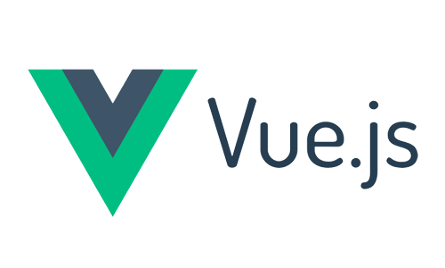
\includegraphics{images/vuejs.png}
\end{figure}

Le module de la maintenance est un nouveau module à développer en MCA. L’équipe technique de 
Clalrisys Informatique a choisi le Framework VueJS pour le développement de la nouvelle 
interface utilisateurs de MCA pour les nouvelles versions à sortir Notamment la versions 9.0.

Evan You\footnote[13]{Evan you est un développeur open source indépendant, 
un designer et un codeur créatif. Il est l'auteur de Vue. js, un framework 
JavaScript permettant de créer des interfaces web modernes avec des composants réactifs.} 
a créé VueJS alors qu’il travaillait chez Google en tant que technologue créatif. 
Ainsi, à certains égards, il est similaire à AngularJs, le framework JavaScript de Google.
VueJS est décrit comme « un framework progressif pour la création d’interfaces utilisateur ». 
Ce qui différencie ce framework des autres frameworks de développement web JavaScript est que son 
architecture est conçue pour être adaptable de manière incrémentielle.

L’écosystème VueJS se compose d’une bibliothèque de base, de frameworks et d’autres outils qui 
permettent un développement front-end facile et rapide. Bien que Vue, lui-même, soit léger et 
minimaliste, il donne tous les outils aux développeurs pour créer des applications web très fonctionnelles.

Le plus grand avantage de VueJS est sa facilité d’intégration dans un projet Web existant. 
Le passage à ce framework est donc très facile et avantageux pour un environnement de développement rapide.

L’un des principaux avantages de VueJS est sa petite taille. L’utilisateur n’a pas
besoin de beaucoup de temps pour télécharger et utiliser ce framework car il ne fait que 
18-21 Ko. Toutefois, cette petite taille ne signifie pas une vitesse inférieure car, 
au contraire, il bat tous ses rivaux volumineux comme Angular, React.JS et Ember.JS.
\pagebreak
